\begin{questions}
\question{
Bravais lattice of Cairo tiling
}
\begin{solution} We can see the found Bravais lattice in fig. \ref{cell}. We can spot it easily, by only joining the intersection points of the tiles making right angles.

  \begin{center}
    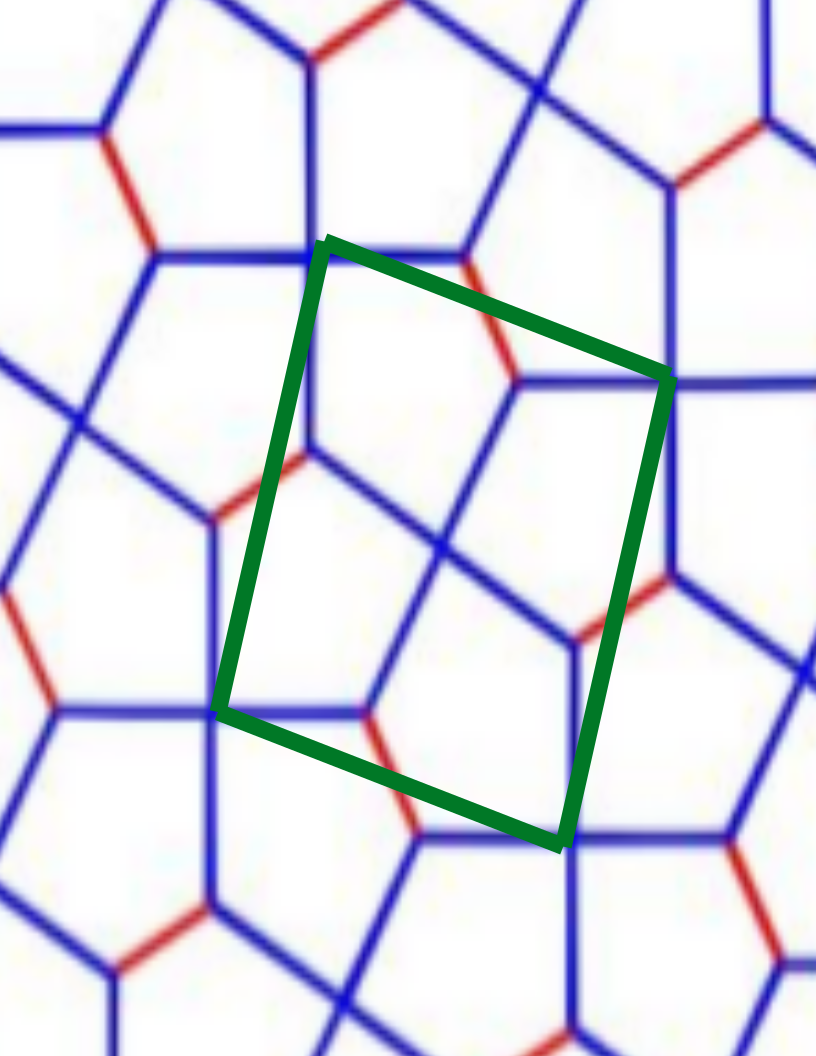
\includegraphics[width=35mm]{cairo_cell}
  \end{center}

  \captionof{figure}{Cell of the Bravais lattice for Cairo tiling}\label{cell}\vspace{0.5cm}

\end{solution}

\question{Primitive cell vectors and angle between them}
\begin{solution}
  The desired elements are shown in fig. \ref{angles}, the angle $\phi$ will be used on the next question.

  \begin{center}
    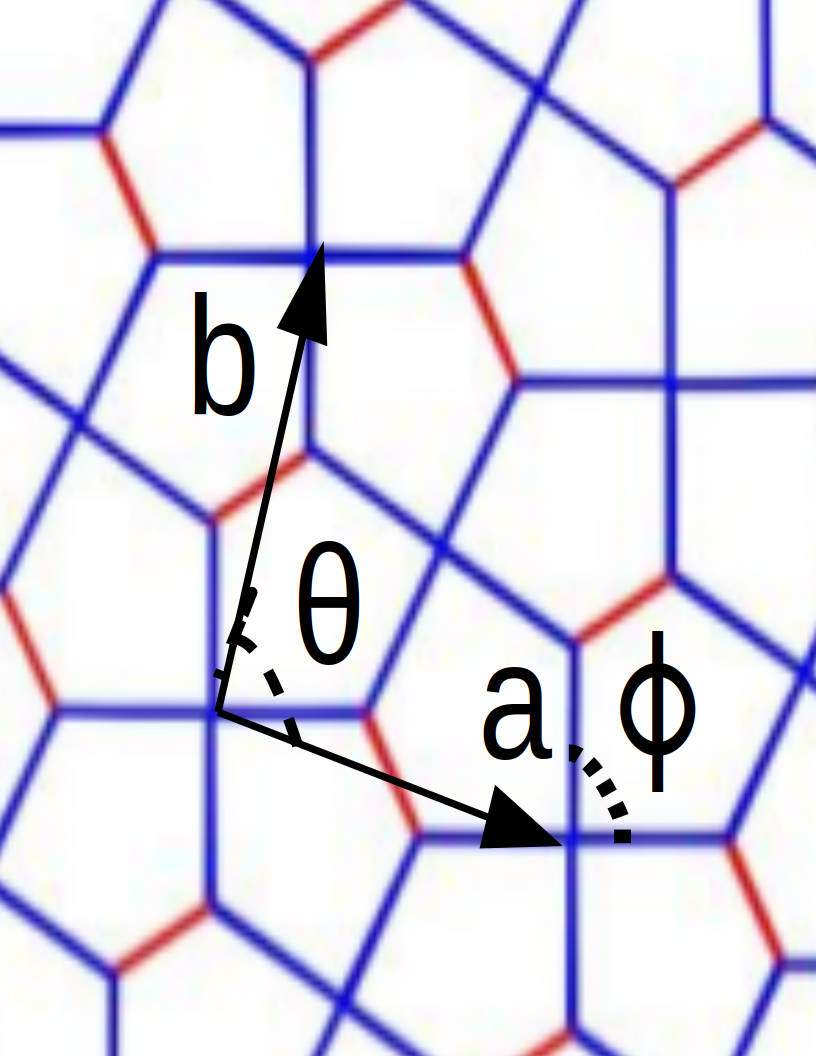
\includegraphics[width=35mm]{angles}
  \end{center}

  \captionof{figure}{Primitive vectors and angle between them on the unit cell of Cairo Tilings}\label{angles}\vspace{0.5cm}
\end{solution}

\question{Determine the value of $\theta$}
\begin{solution}
  It's easy to show, by using corresponding angles, that $\theta = \phi$, and since $\phi = \pi/2$ we have by transitivity that $\hlgreen{\theta = \pi/2}$
\end{solution}

\question{Tilings inside a unit cell}
\begin{solution}
  There are \textbf{4 tiles within a unit cell}.
\end{solution}
\end{questions}

%
% \begin{center}
%   \includegraphics[width=55mm]{}
% \end{center}
%
% \captionof{figure}{}\label{new}\vspace{0.5cm}
